\subsubsubsection*{Segmentação}
\label{sec:segmentacao}

O estudo de segmentação semântica dentro da área de redes neurais convolucionais têm três principais nichos, sendo eles: segmentação semântica que é a classificação por pixel, a segmentação de instância que atribui um id para cada objeto encontrado de uma classe, e a segmentação panóptica que junta as duas anteriores para criar uma imagem semelhante a saída de segmentação semântica porém separando objetos de mesma classe sendo essa a mais recente e completa, a diferença entre esses três tipos está ilustrado na \cref{fig:segentacoes} \space\cite{dp_semantic_segmantation, lapix}.

\begin{figure}[ht]
	\caption{Tipos de segmentação em redes neurais convolucionais}
	\centering % para centralizarmos a figura
	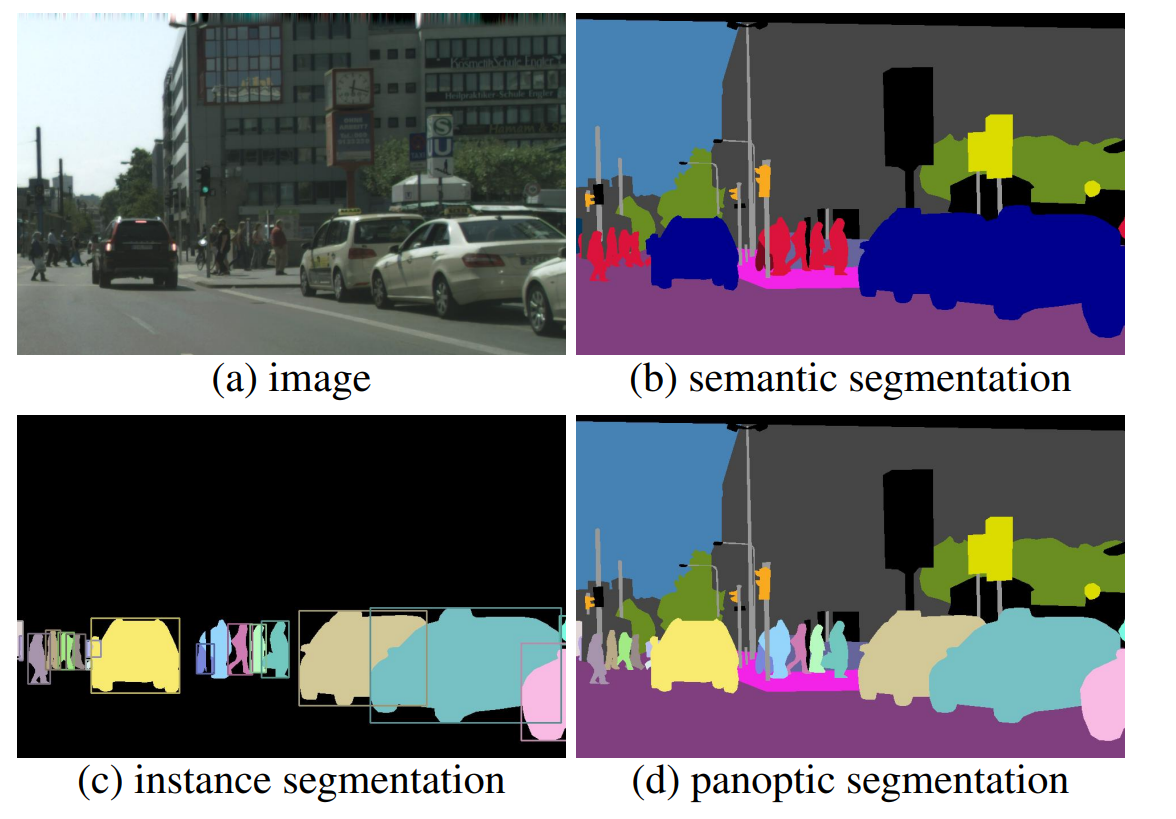
\includegraphics[width=10cm]{figures/segmantations.png} % leia abaixo
	\legend{Fonte: \citeonline{kirillov2019panoptic}}
	\label{fig:segentacoes}
\end{figure}

\subsubsubsection*{Segmentação semântica}

A segmentação semântica começou a ter resultados satisfatórios a partir de redes totalmente convolucionais, com o objetivo de segmentar imagens classificando pixels, esse modelo descarta a camada totalmente conectada pois a saída deverá ser uma imagem e não uma classificação — isso a torna mais rápida para treinar do que as redes neurais convolucionais —, logo usa camadas deconvolucionais para transformar a matriz de características em uma imagem de qualquer dimensão na saída. A RTC criou a arquitetura chamada de salto (ou conexões) que serve para evitar perdas em camadas de agrupamento criando conexões entre camadas não consecutivas — geralmente entre camadas convolucionais e deconvolucionais — como apresentado na \cref{fig:rtc}, a arquitetura de salto evoluiu para arquitetura codificador-decodificador.
\begin{figure}[ht]
	\caption{Exemplo de arquitetura de rede totalmente convolucional}
	\centering % para centralizarmos a figura
	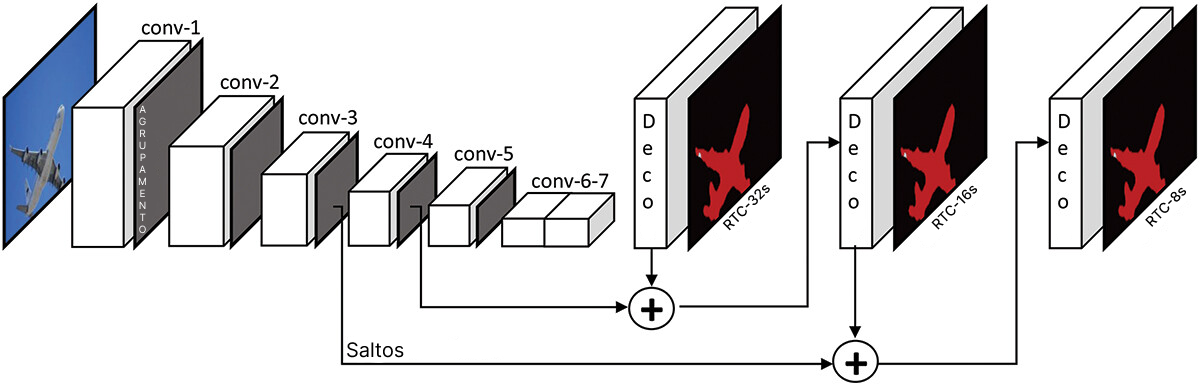
\includegraphics[width=10cm]{figures/redes_totalmente_convolucionais.png} % leia abaixo
	\legend{Fonte: \citeonline{dp_semantic_segmantation}}
	\label{fig:rtc}
\end{figure}

A arquitetura codificador-decodificador — ou Encoder-Decoder —, é separada em dois passos: o primeiro para convergir no mapa de características — chamado de codificador — e o segundo para reverter — chamado de decodificador — as camadas de agrupamento para aumentar a dimensão da saída, usando camadas deconvolucionais e de desagrupamento. Outra característica importante é a conexão entre camadas de mesmo nível, como por exemplo a arquitetura UNet, que foi a primeira a implementar o padrão Codificador-Decodificador. Na \cref{fig:unet} pode-se observar que tem formato da letra U, sendo a descida a parte de codificação e subida decodificação \space\cite{dp_semantic_segmantation, lapix, unetArq}.

\begin{figure}[ht]
	\caption{Arquitetura codificador-decodificador UNet}
	\centering % para centralizarmos a figura
	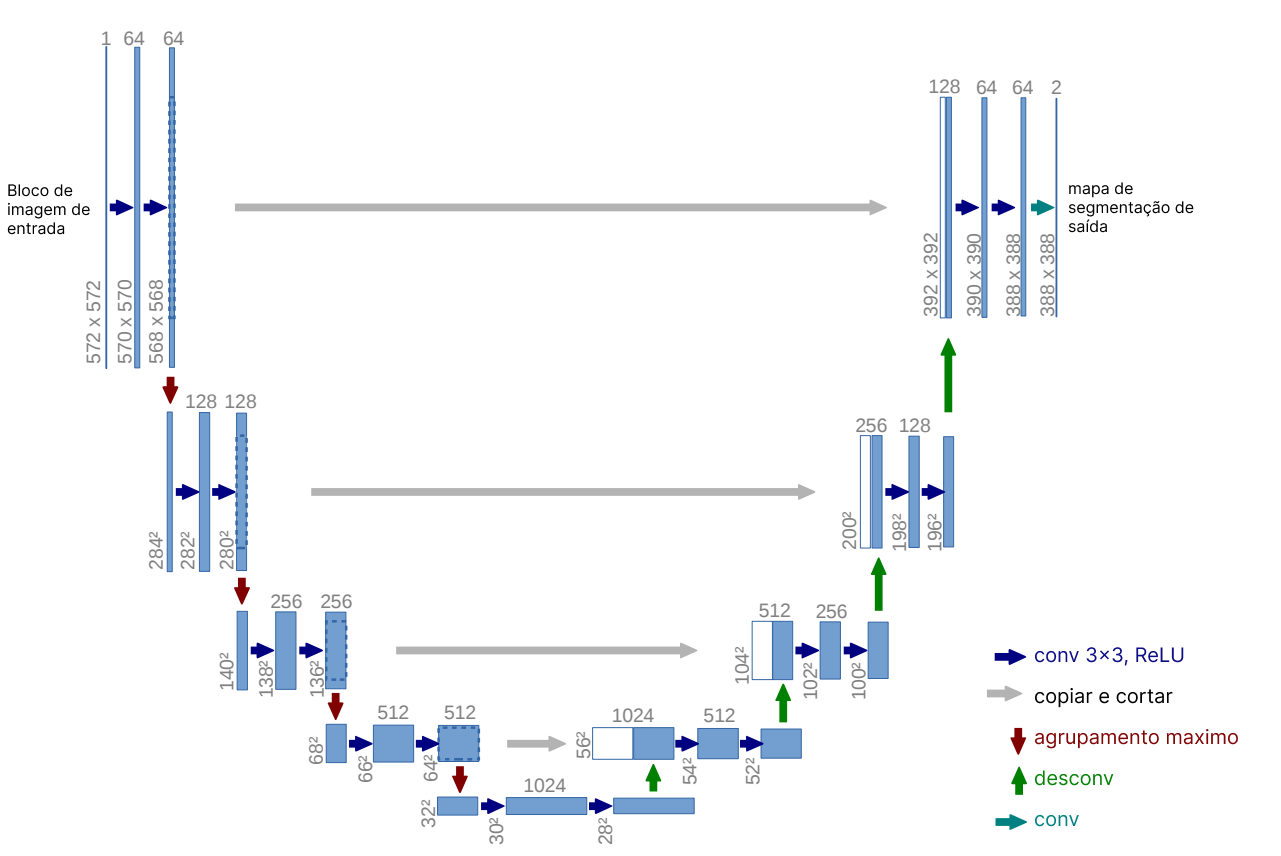
\includegraphics[width=10cm]{figures/unet.png} % leia abaixo
	\legend{Fonte: \citeonline{unetArq}}
	\label{fig:unet}
\end{figure}

\subsubsubsection*{Segmentação de instância}

Outro problema dentro da área de visão computacional é a detecção de objetos, a primeira solução foi com Características de regiões com RNC — Regions with CNN features (R-CNN) — que se resume em dividir a imagem de entrada em regiões de interesse e nessas regiões aplicar uma RNC. A arquitetura que seleciona essas regiões é chamada de Rede de Proposta de Região (RPR) — ou Region Proposal Network (RPN) — o que auxilia na detecção por caixas delimitadoras. Essa ideia inicial foi estendida para segmentação de instância criando também máscara nos objetos, como por exemplo a arquitetura Mask R-CNN \space\cite{dp_semantic_segmantation, lapix}.

A arquitetura Mask R-CNN é derivado do Fast R-CNN — aprimoramento do R-CNN aplicando conceito RoIPool para classificar — onde há uma segmentação de máscara em cada RoI — ou Região de interesse — paralela com a classificação da caixa delimitadora. A máscara é classificada com uma pequena RTC em cada RoI. Além de ter uma pequena melhoria na RoIPool, pois havia um problema de alinhamento nas localizações espaciais exatas, essa camada é chamada de RoIAlign \space\cite{maskRCNN}.

\subsubsubsection*{Segmentação panóptica}

Um problema encontrado na segmentação semântica é que objetos de mesma classe não são separados como na segmentação de instância, logo surgiu uma ideia para criar uma solução usando as duas técnicas. Esse conceito surgiu do trabalho \citeonline{kirillov2019panoptic} e consiste na definição geral da ideia, uma métrica — que será explicada posteriormente — unificada para classificar os resultados do modelo além de fazer a distinção entre coisas — ou stuff — que não são contáveis, como o céu e os objetos — ou things — que são contáveis como carros, pessoas, etc.
Os principais conjunto de dados para tarefa panóptica são COCO-Panoptic, Cityscapes, Mapillary Vistas, ADE20K, e Indian Driving Dataset. Cada conjunto de dados possui diversas classes para o modelo aprender \space\cite{v7labs2022panoptic}.

\subsubsubsection*{Métricas e técnicas}
\label{sec:metricas_tecnicas}

No ramo de segmentação existem diversas métricas que podem ser usadas, dentre elas algumas serão destacas nesta monografia a seguir:

\subsubsubsection*{Classificação de conjuntos}
\label{sec:classificacao_conjuntos}

A classificação de conjuntos é uma técnica para criar relações entre a imagem de predição e a imagem do conjunto de dados. Ela se divide em quatro conjuntos sendo eles: Positivo Verdadeiro — ou True Positive(TP) —
% sendo o requisito ter uma intersecção significativa entre classes iguais, \emph{i.e.}, IoU > 0.5
, Negativo Verdadeiro — ou True Negative(TN) —, Falso Positivo — ou False Positive(FP) — quando um objeto não é correspondido na imagem de predição e por fim o Falso Negativo — ou False Negatives(FN) — quando um objeto não é correspondido na imagem do conjunto de dados. Essa técnica pode ser usada em modelos de classificação binária usando uma matriz de confusão mas na área de segmentação costuma-se contar os pixeis e sua representação visual pode-se observar na \cref{fig:conjuntos} \space\cite{kirillov2019panoptic, Wang2020}.
\begin{figure}[ht]
	\caption{Exemplo da classificação dos conjuntos usados nas métricas de segmentação}
	\centering % para centralizarmos a figura
	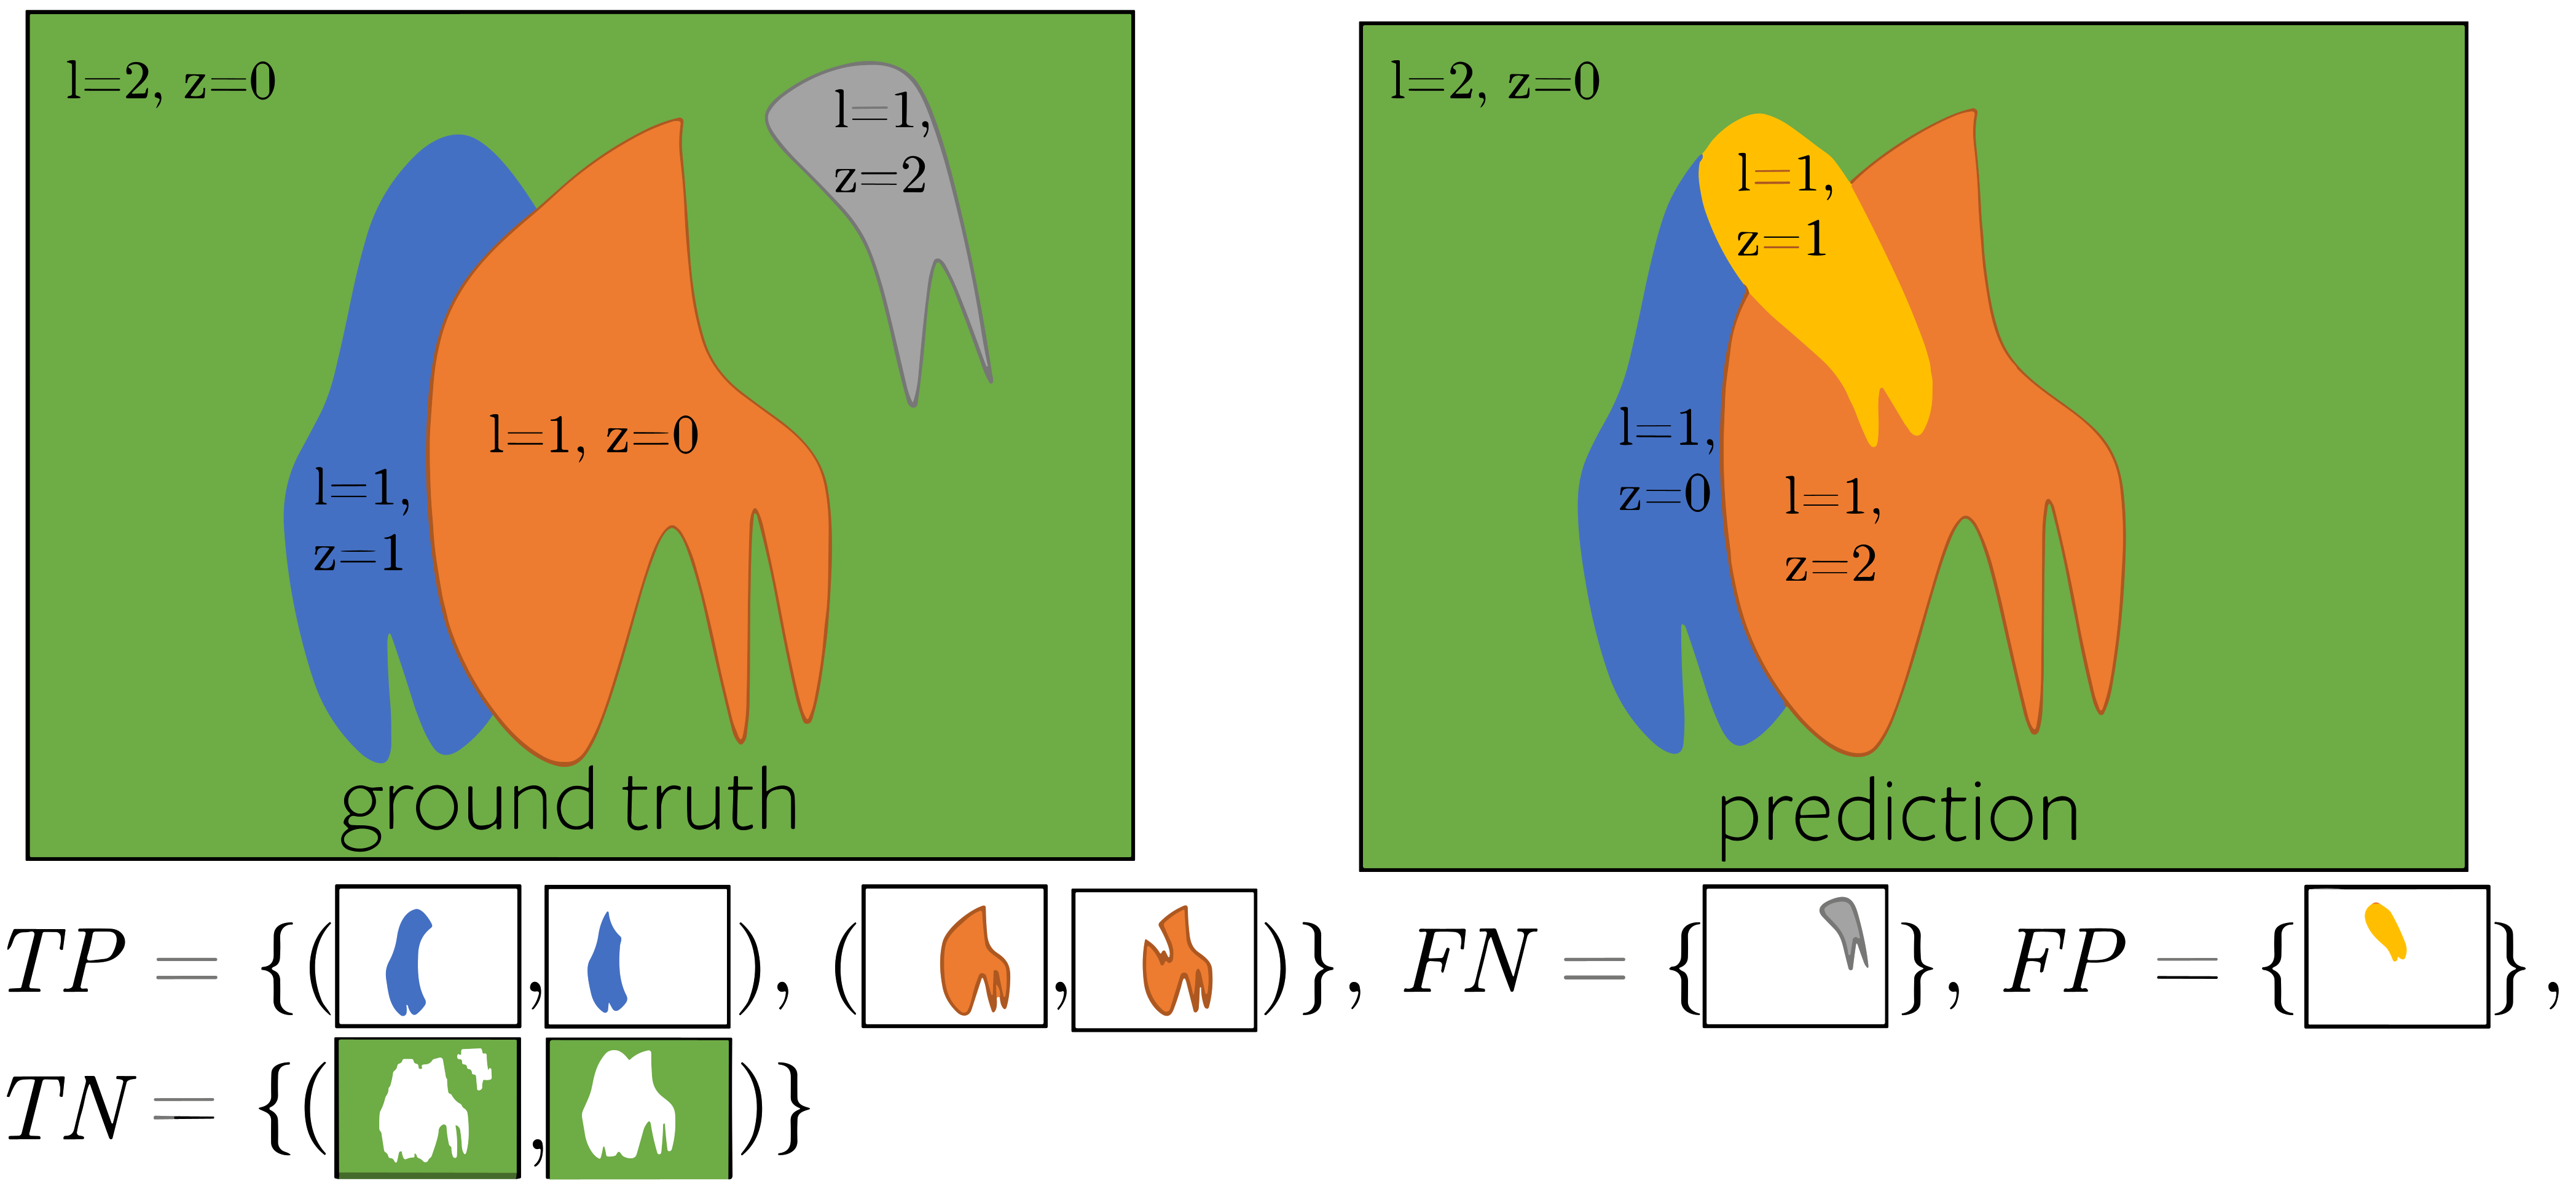
\includegraphics[width=15cm]{figures/pan_metric.png} % leia abaixo
	\legend{Fonte: \citeonline{slidesKirillov} editado}
	\label{fig:conjuntos}
\end{figure}


\subsubsubsection*{F1 Score}

O F1 Score é uma métrica que pode ser utilizada para calcular a eficiência de modelos de segmentação de instância,  baseando-se em encontrar uma relação entre a área das classes da imagem de saída com as classes na imagem do conjunto de dados porém diminuindo o peso dos erros. Varia de 0 a 1 sendo 1 com maior eficiência. Segue a exemplificação da \cref{eq:f1} \space\cite{Chicco2020}:

\begin{equation}
	\label{eq:f1}
	F1\ Score = \frac{\text{TP}}{(TP + \frac{FP}{2} + \frac{FN}{2} )}
\end{equation}

\subsubsubsection*{Coeficiente de correlação de Matthews}

O coeficiente de correlação de Matthews — ou Matthews Correlation Coefficient (Mcc) —  é uma métrica que pode ser utilizada para mensurar a eficiência de modelos de segmentação,  baseando-se no coeficiente de correlação de Pearson. Varia de -1 a 1 sendo 1 com maior correlação, 0 inconclusivo e -1 sem correlação. Segue a exemplificação da \cref{eq:mcc} \space\cite{Chicco2020, confusion_matrix_calculator}:

\begin{equation}
	\label{eq:mcc}
	Mcc = \frac{\text{TP}\cdot\text{TN}-\text{FP}\cdot\text{FN}}{\sqrt{ (\text{TP}+\text{FP})\cdot(\text{TP}+\text{FN})\cdot(\text{TN}+\text{FP})\cdot(\text{TN}+\text{FN}) }}
\end{equation}

\subsubsubsection*{Taxa de descoberta falsa}

A taxa de descoberta falsa — ou False Discovery Rate (FDR) — é uma métrica utilizada para calcular o erro obtido na imagem de predição,  baseando-se em encontrar uma relação entre ao erro obtido, divido pelo erro mais acerto esperado. Varia de 0 a 1 sendo 1 o pior caso e 0 o melhor. Segue a exemplificação da \cref{eq:fdr} \space\cite{confusion_matrix_calculator}:

\begin{equation}
	\label{eq:fdr}
	Fdr = \frac{FP}{FP + TP}
\end{equation}


\subsubsubsection*{Taxa de Falso Negativo}

A taxa de falso negativo — ou False Negative Rate (FNR) — é uma métrica utilizada para calcular o erro obtido na imagem verdade,  baseando-se em encontrar uma relação entre ao erro obtido, divido pelo erro mais acerto esperado. Varia de 0 a 1 sendo 1 o pior caso e 0 o melhor. Segue a exemplificação da \cref{eq:fnr} \space\cite{confusion_matrix_calculator}:

\begin{equation}
	\label{eq:fnr}
	Fnr = \frac{FN}{FN + TP}
\end{equation}

\subsubsubsection*{Acurácia}

A acurácia — ou Accuracy (Acc) — é uma métrica utilizada para calcular a eficiência de modelos de segmentação semântica,  baseando-se em encontrar uma relação entre a área das classes da imagem de saída com as classes na imagem do conjunto de dados para todos conjuntos. Varia de 0 a 1 sendo 1 com maior eficiência. Segue a exemplificação da \cref{eq:acc} \space\cite{Chicco2020}:

\begin{equation}
	\label{eq:acc}
	Acc = \frac{\text{TP + TN}}{\text{(TP + TN + FP + FN)}}
\end{equation}

\subsubsubsection*{União sobre intersecção}

A união sobre intersecção — ou Intersection over Union (IoU) — ou índice de Jaccard é uma métrica muito utilizada para calcular a eficiência de modelos de segmentação, ela se baseia em encontrar uma relação entre a área das classes da imagem de saída com as classes na imagem do conjunto de dados para qualquer valor positivo, isto é, desconsiderando o conjunto positivo falso. Varia de 0 a 1 sendo 1 com maior eficiência. Segue a exemplificação da \cref{eq:iou} \space\cite{iou_metric_link}:

\begin{equation}
	\label{eq:iou}
	IoU = \frac{\text{TP}}{\text{(TP + FP + FN)}}
\end{equation}

\subsubsubsection*{Qualidade panóptica}

A qualidade panóptica — ou Panoptic Quality (PQ) — foi definido pela primeira vez no artigo \citeonline{kirillov2019panoptic}, e se resume na fórmula:

\begin{equation}
\label{eq:pq_metric}
PQ = \frac{\sum_{(p,g)\in TP}IoU(p,g)}{ |TP| + \frac{1}{2}|FP| + \frac{1}{2}|FN|}
\end{equation}

Multiplicando a \cref{eq:pq_metric} por $\frac{|TP|}{|TP|}$ tem-se:

\begin{equation}
	\label[]{eq:pq_metric_mult}
	PQ = \underbrace{\frac{\sum_{(p,g)\in TP}IoU(p,g)}{|TP|}}_{\text{Segmentation Quality (SQ)}}
	\times
	\underbrace{\frac{|TP|}{|TP| + \frac{1}{2}|FP| + \frac{1}{2}|FN|}}_{\text{Recognition Quality (RQ)}}
\end{equation}

Portanto pode-se concluir que PQ é apenas uma simplificação para uma fórmula que contém uma relação entre métricas de segmentação semântica e de instância.

Com base no subtópico \hyperref[sec:segmentacao]{Segmentação} percebe-se que a segmentação panóptica é a mais completa e por efeito de estudos será utilizado o mesmo para concluir o trabalho. Como nesse nicho existem várias alternativas será utilizado a métrica demonstrada na \cref{eq:pq_metric} para analisar resultados e selecionar o modelo.

\subsubsubsection*{Resultados de modelos do nicho de segmentação panóptica}

Os resultados são de uma competição em aberto criada pela Cityscapes Dataset, essa competição tem várias modalidades e esses são referentes ao nicho de segmentação panóptica utilizando a métrica PQ na classe de pessoas. A exibição dos resultados contendo a métrica PQ que classifica pessoas com os quinze melhores modelo encontra-se na \cref{tab:resultados-cityscapes} \space\cite{datasetResults}.
\begin{table}[h]
	\centering
	\caption{Top 15 modelos que melhor classificam pessoas com métrica P em segmentação panóptica}
	\label{tab:resultados-cityscapes}
	\begin{tabular}{|l|c|}
	  \hline
	  Nome do modelo & PQ (\%) \\
	  \hline
	  EfficientPS [Mapillary Vistas] & 61,6 \\
	  EfficientPS [Cityscapes-fine] & 60,9 \\
	  Panoptic-DeepLab w/ SWideRNet [Mapillary Vistas + Pseudo-labels] & 60,6 \\
	  hri\_panoptic & 60,6 \\
	  Naive-Student (iterative semi-supervised learning with Panoptic-DeepLab) & 60,2 \\
	  Panoptic-DeepLab w/ SWideRNet [Mapillary Vistas] & 59,8 \\
	  iFLYTEK-CV & 59,2 \\
	  Panoptic-DeepLab [Mapillary Vistas] & 58,5 \\
	  Panoptic-DeepLab w/ SWideRNet [Cityscapes-fine] & 58,4 \\
	  Seamless Scene Segmentation & 57,7 \\
	  Axial-DeepLab-XL [Mapillary Vistas] & 57,2 \\
	  Unifying Training and Inference for Panoptic Segmentation [COCO] & 56,5 \\
	  kMaX-DeepLab [Cityscapes-fine] & 56 \\
	  Axial-DeepLab-L [Mapillary Vistas] & 55,9 \\
	  TASCNet-enhanced & 55,2 \\
	  \hline
	\end{tabular}
  \end{table}



